% !TeX spellcheck = it_IT
\newpage
\section{Cache}
La cache memory è la memoria più vicina al processore, solitamente sono le SRAM, ma alcune volte sono implementate anche come DRAM. Ad oggi tutte le architetture hanno alcuni livelli di cache integrati nel chip, essa può essere più o meno grande e può avere più di un livello.

\subsection{Gestione del movimento dei dati}
Fra il primo livello di cache e i registri il trasferimento è gestito dal compilatore. Il trasferimento fra caches e RAM viene invece gestito dalla microarchitettura. Infine la gestione dei trasferimenti fra RAM e storage viene fatta dal sistema operativo.

\begin{figure}[h!]
	\centering
	\begin{subfigure}{.45\textwidth}
		\centering
		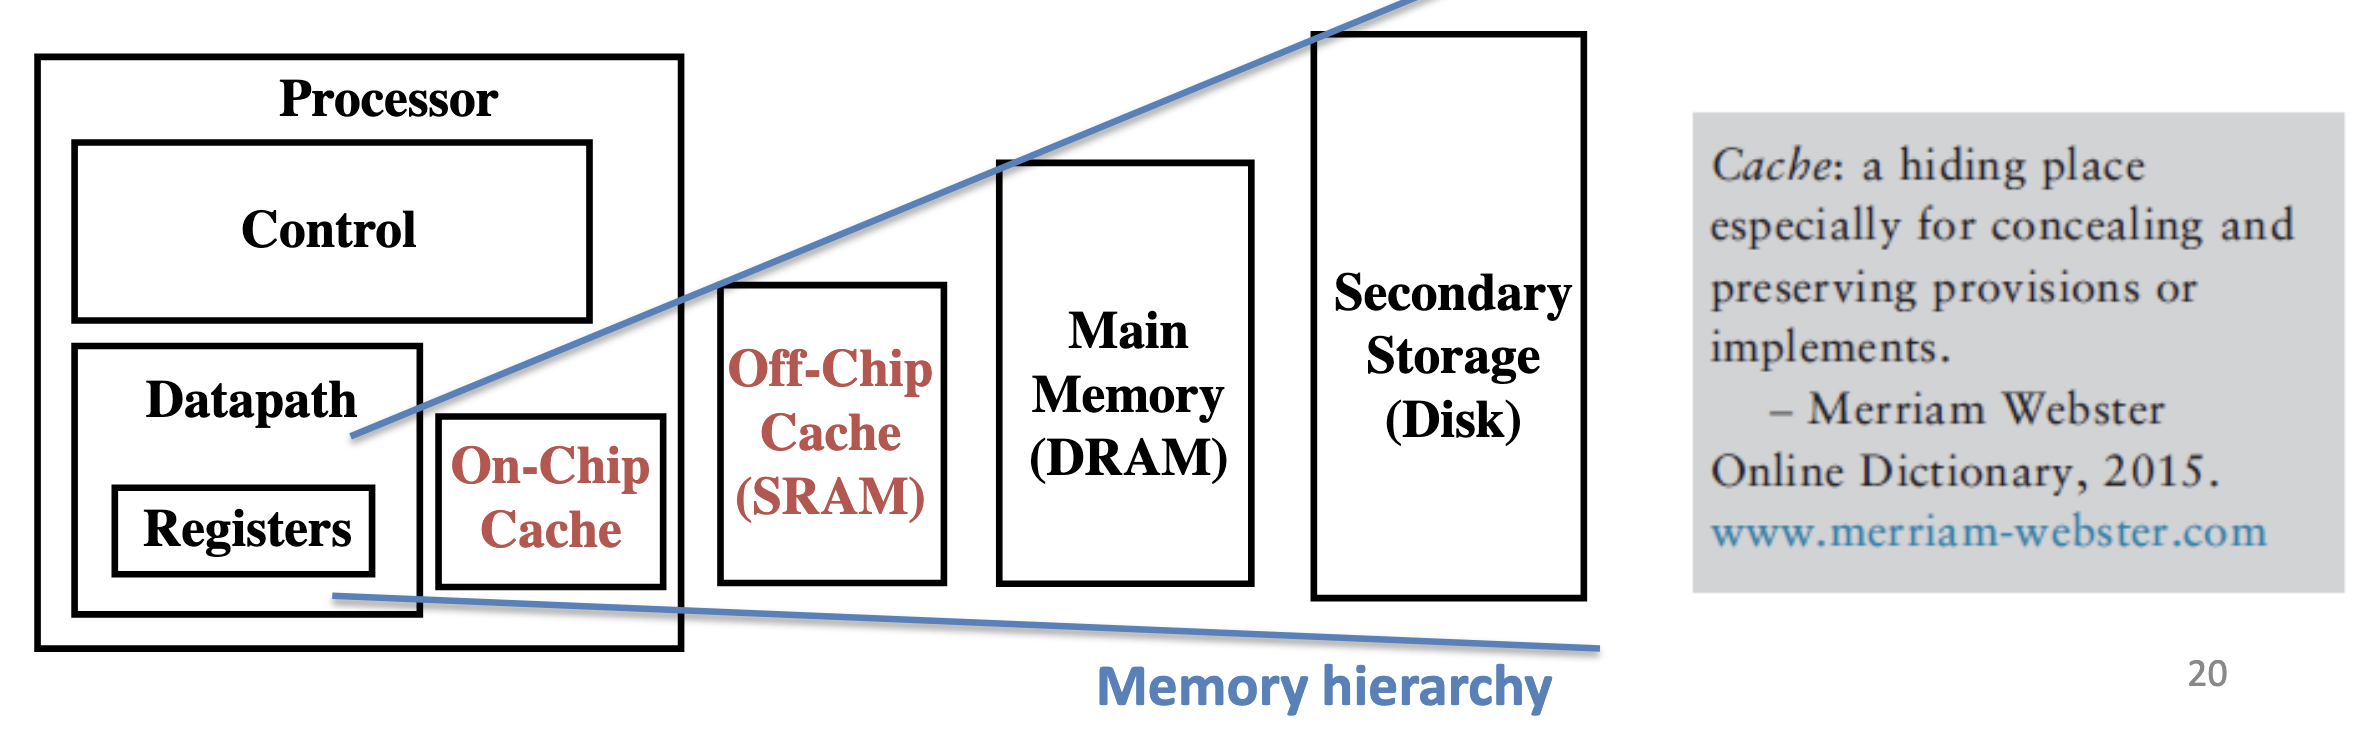
\includegraphics[width=6.5cm]{images/cache-memories.png}
		\caption{}
	\end{subfigure}
	\begin{subfigure}{.45\textwidth}
		\centering
		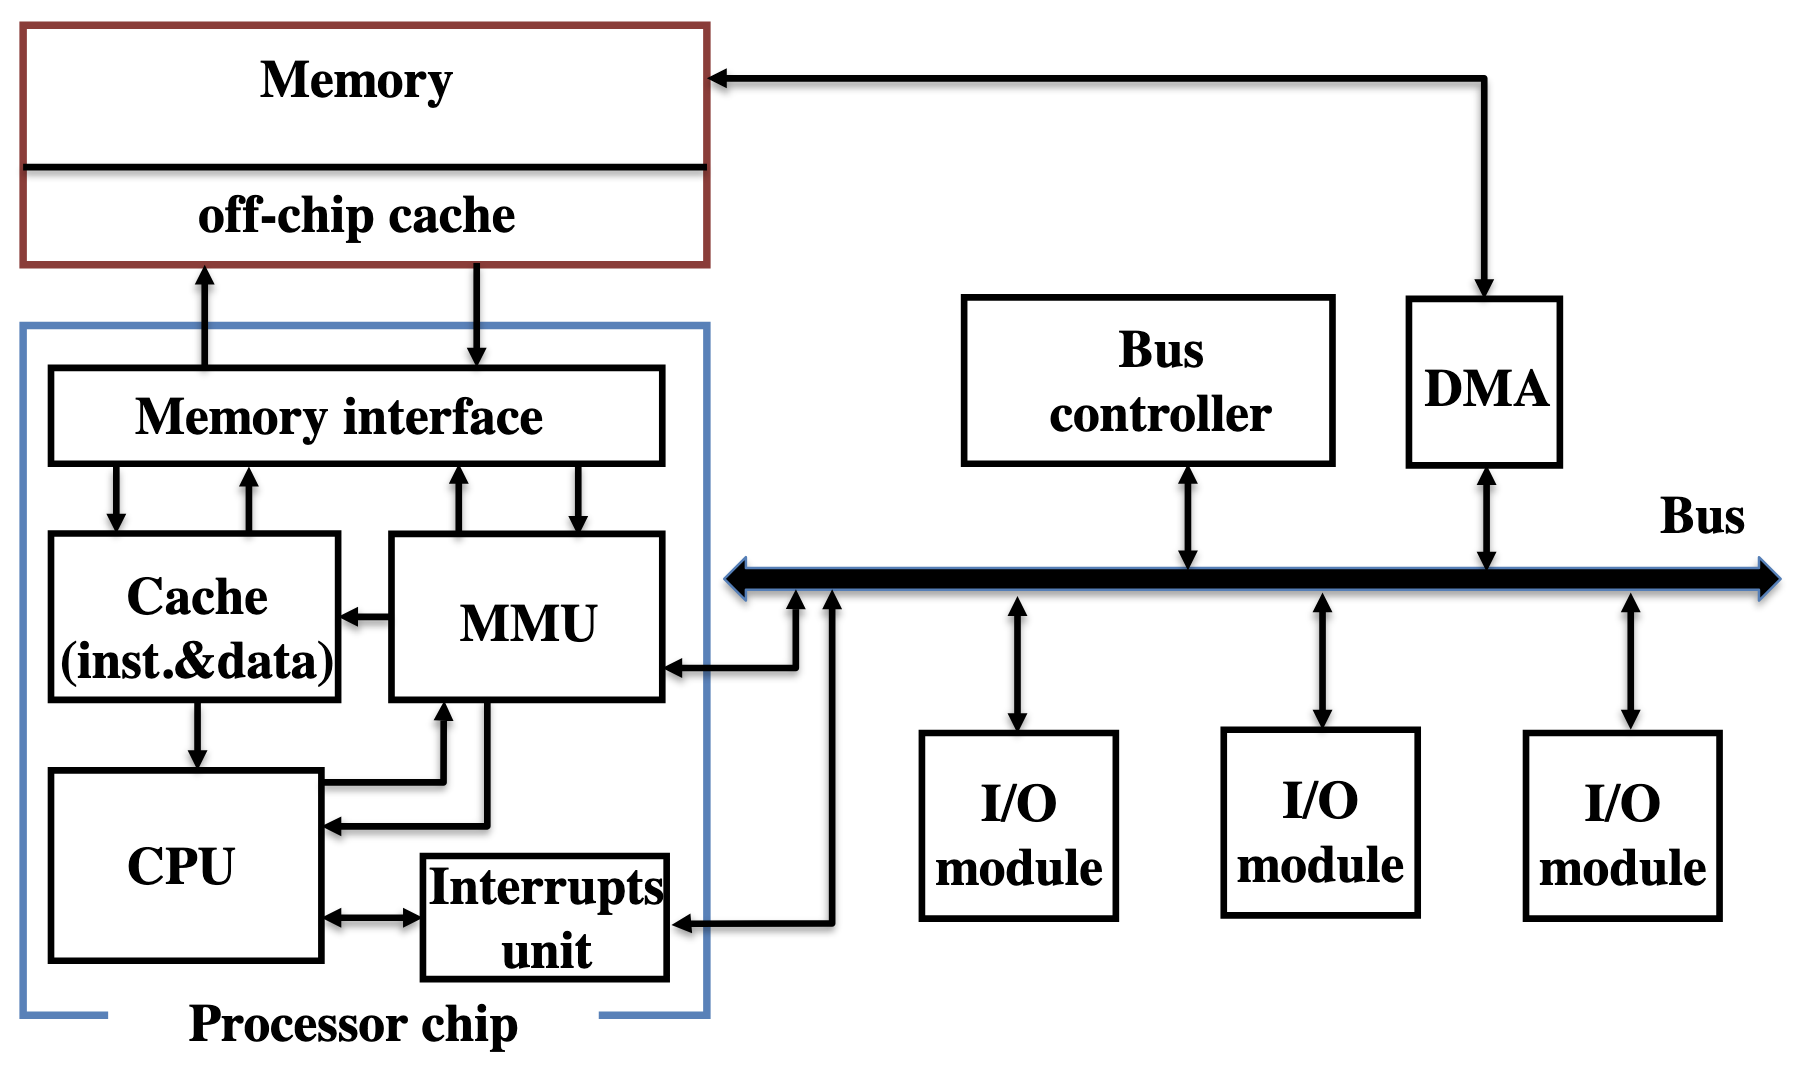
\includegraphics[width=6.5cm]{images/cache-based-architecture.png}
		\caption{}
	\end{subfigure}
\end{figure}


\subsection{Utilizzo}
L'organizzazione della cache avviene non a blocchi ma a linee. Ogni linea contiene blocchi di memoria (8-16 memory words). La prima volta che il processore richiede la memory word avviene una \textbf{cache miss}. A quel punto il blocco contenente la parola viene trasferito dentro la cache.\\
La richiesta successiva può essere di due tipologie:
\begin{itemize}
	\item \textbf{Cache hit}: se il dato è presente nel blocco.
	\item \textbf{Cache miss}: se il dato non è presente dentro il blocco. In questo caso il blocco che contiene il dato viene trasferito dentro la cache line.
\end{itemize}

Vediamo ora l'effetto della cache sull'AMAT. Innanzitutto l'utilizzo di grandi cache nella gerarchia delle memorie aiuta a ridurre il bottleneck di von Neumann. 
\begin{example}
	Vediamo un esempio quantitativo stabilendo dei valori:\\
	$t_M = 50ns$ (main memory service time), $t_{L1} = 1ns$ (L1 hit time, cache hit service time). \\\\
	Abbiamo un Miss rate ($MR_{L1}$) del $5\%$.\\
	Senza cache $AMAT = 50ns$ mentre con L1 cache $AMAT = t_{L1} + MR_{L1} * t_M = 1 + 0.05 * 50 = 3.5ns$
\end{example}

\subsection{Performance}
\begin{equation}
	CPU_{time} = \text{ClockCycles} \cdot \text{ClockCycleTime} = IC \cdot CPi \cdot \text{ClockCyleTime}
\end{equation}
dove
\begin{itemize}
	\item \textbf{IC} (Instruction Count) è il numero di istruzioni che vengono effettivamente eseguite
	\item \textbf{CPI} (ClockCycles Per Instruction) è definito come \(\frac{clockcycles}{IC}\)
\end{itemize}
Possiamo inoltre dividere il $CPU_{time}$ tra \textbf{$CPI_{Perfect}$}, ovvero il tempo che la CPU impiega per eseguire un'istruzione senza \emph{misses}, e \textbf{$CPI_{Stall}$}, ovvero il tempo che la CPU impiega per aspettare la memoria.
\begin{equation}
	CPU_{time} = (CPI_{Perfect} + CPI_{Stall}) \cdot \text{ClockCycleTime}
\end{equation}
Le due parti le possiamo calcolare come segue:
\begin{equation}
	\begin{split}
		CPI = \bigg(\frac{IC_{CPU}}{IC}\bigg) \cdot CPI_{CPU} + \bigg(\frac{IC_{MEM}}{IC}\bigg) \cdot CPI_{MEM} \\
		CPI_{MEM} = CPI_{MEM-HIT} + \text{Miss Rate} \cdot CPI_{MEM-MISS} \\
		\mathbf{CPI_{Perfect}} = \frac{IC_{CPU}}{IC} \cdot CPI_{CPU} + \frac{IC_{MEM}}{IC} \cdot CPI_{MEM-HIT} \\
		\mathbf{CPI_{Stall}} = \frac{IC_{MEM}}{IC} \cdot \text{Miss Rate} \cdot \text{Miss Penalty}
	\end{split}
\end{equation}

\begin{observation}
	IL $CPI_{Stall}$ è definito come la somma dei cicli di stallo in lettura e scrittura. Per semplicità abbiamo assunto che i miss rate e le miss penalties fossero identiche per lettura e scrittura e che gli stalli per scrivere nei buffer fossero trascurabili.
\end{observation}

\begin{example}
	\label{example:cache_performance}
	Assumiamo che abbiamo un miss rate del \(2\%\) per la cache delle istruzioni mentre un \(4\%\) per la cache dei dati, ed una miss penalty di $100$ cicli per ogni mancanza. Una frequenza del \(36\%\) per le \emph{ldr}, e le \emph{str}. Se la CPI è $2$ senza memory stalls, dobbiamo determinare quanto va più veloce un processore con una cache perfetta rispetto ad una cache reale (che ha le caratteristiche elencate sopra).\\
	
	\[CPI_{Stall-Instr} = 1 \cdot 0.02 \cdot 100 = 2 cycles\]
	\[CPI_{Stall-Data} = 0.36 \cdot 0.4 \cdot 100 = 1.44 cycles\]
	\[CPi_{stall} = 2 + 1.44 = 3.44\]
	spendiamo in media $3.44$, e quindi in totale il nostro processore $CPI = 2 + 3.44 = 5.44$.
	
	\[\frac{CPU_{\text{time with stalls}}}{CPU_{time Perfect}} = \frac{(CPI_{Perfect} + CPI_{Stall}) \cdot Clockcycletime}{CPI_{perfect} \cdot ClockCycleTime} =  \frac{5.44}{2}\]
\end{example}

Come abbiamo visto nell'esempio è quindi importante tenere bassi:
\begin{itemize}
	\item \textbf{Hit-time}, che deriva dalla tecnologia utilizzata per la cache
	\item \textbf{Miss penalty}, che deriva dall'architettura utilizzata
	\item \textbf{Miss rate}, che può essere abbassato anche tramite tecniche di programmazione
\end{itemize}

\subsection{Design}
Una delle prime domande che dobbiamo porci è come i dati sono organizzati.\\
Partiamo da una cache di una capacità C, organizzata come S sets in cui ciascuno contiene B block (o linee), dove b è il numero di parole per blocco. Tutto questo in un sistema a $32$bit (quindi al massimo possiamo indirizzare $2^{30}$ parole).\\
Da qui possiamo distinguere vari metodi di organizzazione:
\begin{enumerate}
	\item \textbf{Direct mapped}: in questo caso $\#S=\#B$
	\item \textbf{N-way set-associative}, in cui N definisce il numero di blocchi contenuti in un set quindi $S=B/N$
	\item \textbf{Fully associative}, in cui nell'insieme c'è uno unico blocco contenente tutta la cache, quindi $S=1$
\end{enumerate}

\subsubsection{Direct mapped}
Supponiamo di avere $b=1$\footnote{Nessuna cache avrà mai b=1, è solo come esempio} e una cache di 8 parole, quindi $S=B=8$, $C=B\cdot b=8$. Per indirizzare le 8 parole ci serviranno $\log_2 8 = 3$bits.\\

\begin{wrapfigure}{r}{6.5cm}
	\centering
	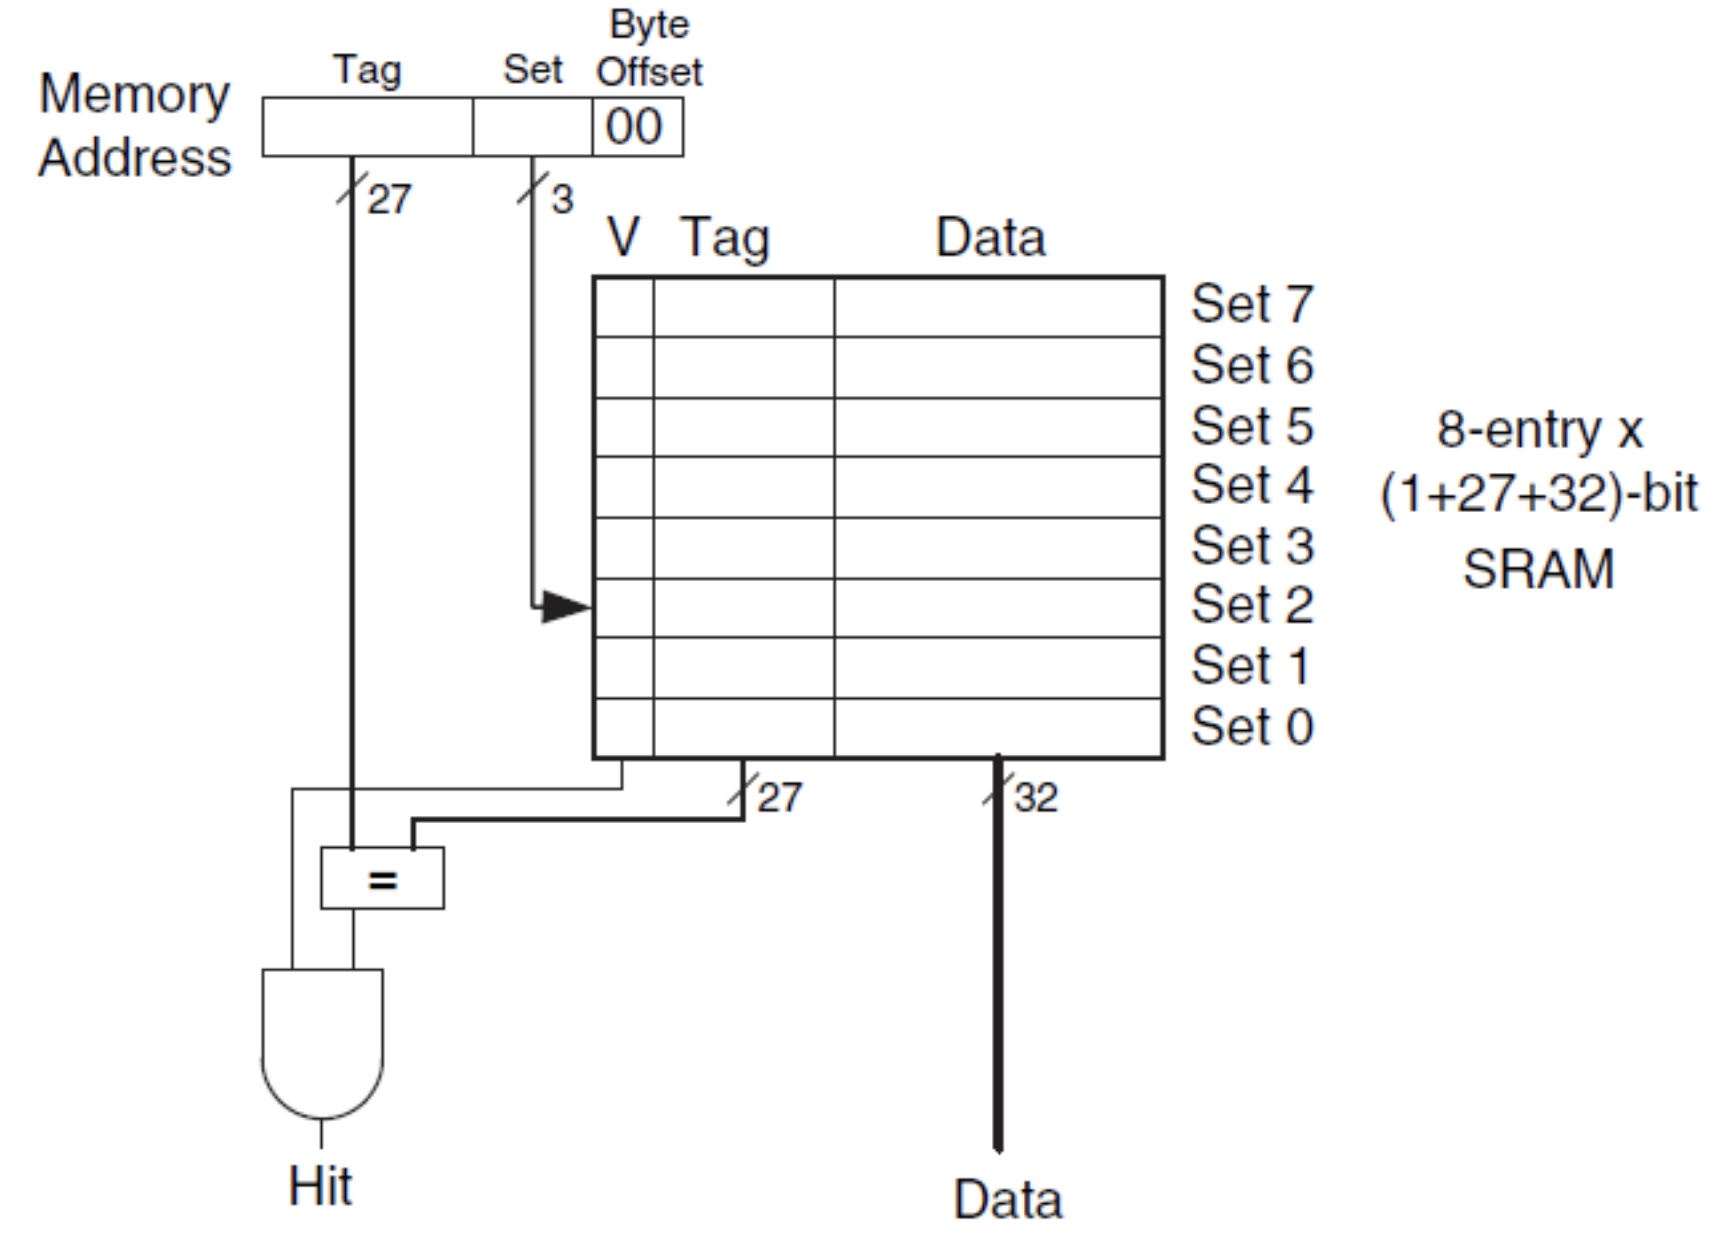
\includegraphics[width=4.5cm]{images/direct-mapped.png}
	\caption{Direct mapped, $b=1$}
\end{wrapfigure}

In questo tipo di design, tutti gli indirizzi con il quintultimo, quartultimo e terzultimo bit in comune saranno associati ad un set nella cache predefinito. \\
In aggiunta nella cache sarà pesente anche un \textbf{tag} che permette di identificare univocamente il dato e un valore di \textbf{controllo} che mi garantisca che quel dato sia effettivamente valido per quella posizione di cache (ad esempio appena acceso il computer potrebbe esserci un valore random non corretto).\\

\noindent Vediamo un caso realistico dove \(b > 1\). Prendiamo $C = 8$ e $b = 4$,con $B = C/b = 2$ e $S = 2$. Dobbiamo quindi andare af "affettare l'indirizzo" aggiungendo un \textbf{block-offset} che mi permetta di selezionare la parola corretta tra le $\log_2 4$ opzioni
\begin{center}
	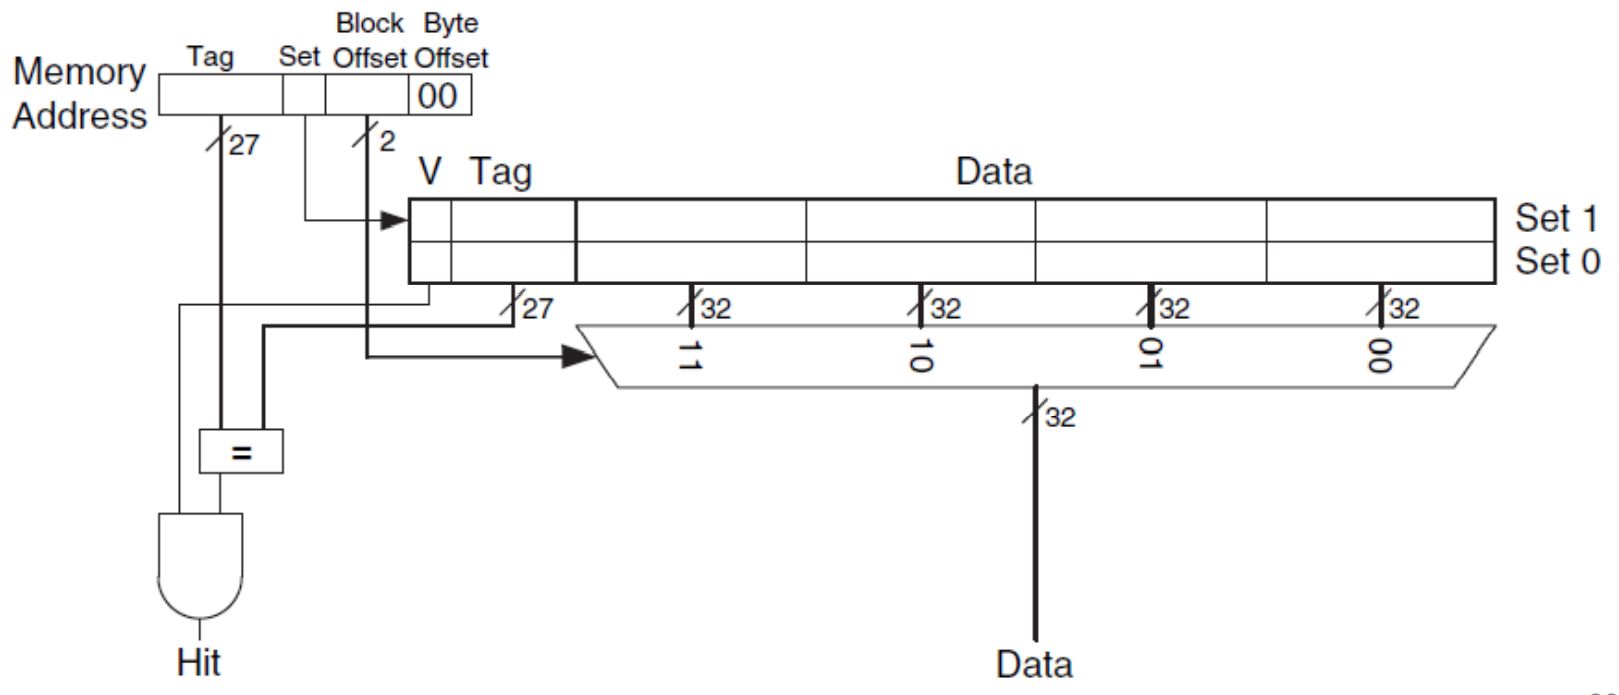
\includegraphics[scale=0.15]{images/direct_mapped_2.png}
\end{center}

\noindent Per implementare anche la scrittura in un indirizzo, aggiorniamo lo schema come segue:
\begin{center}
	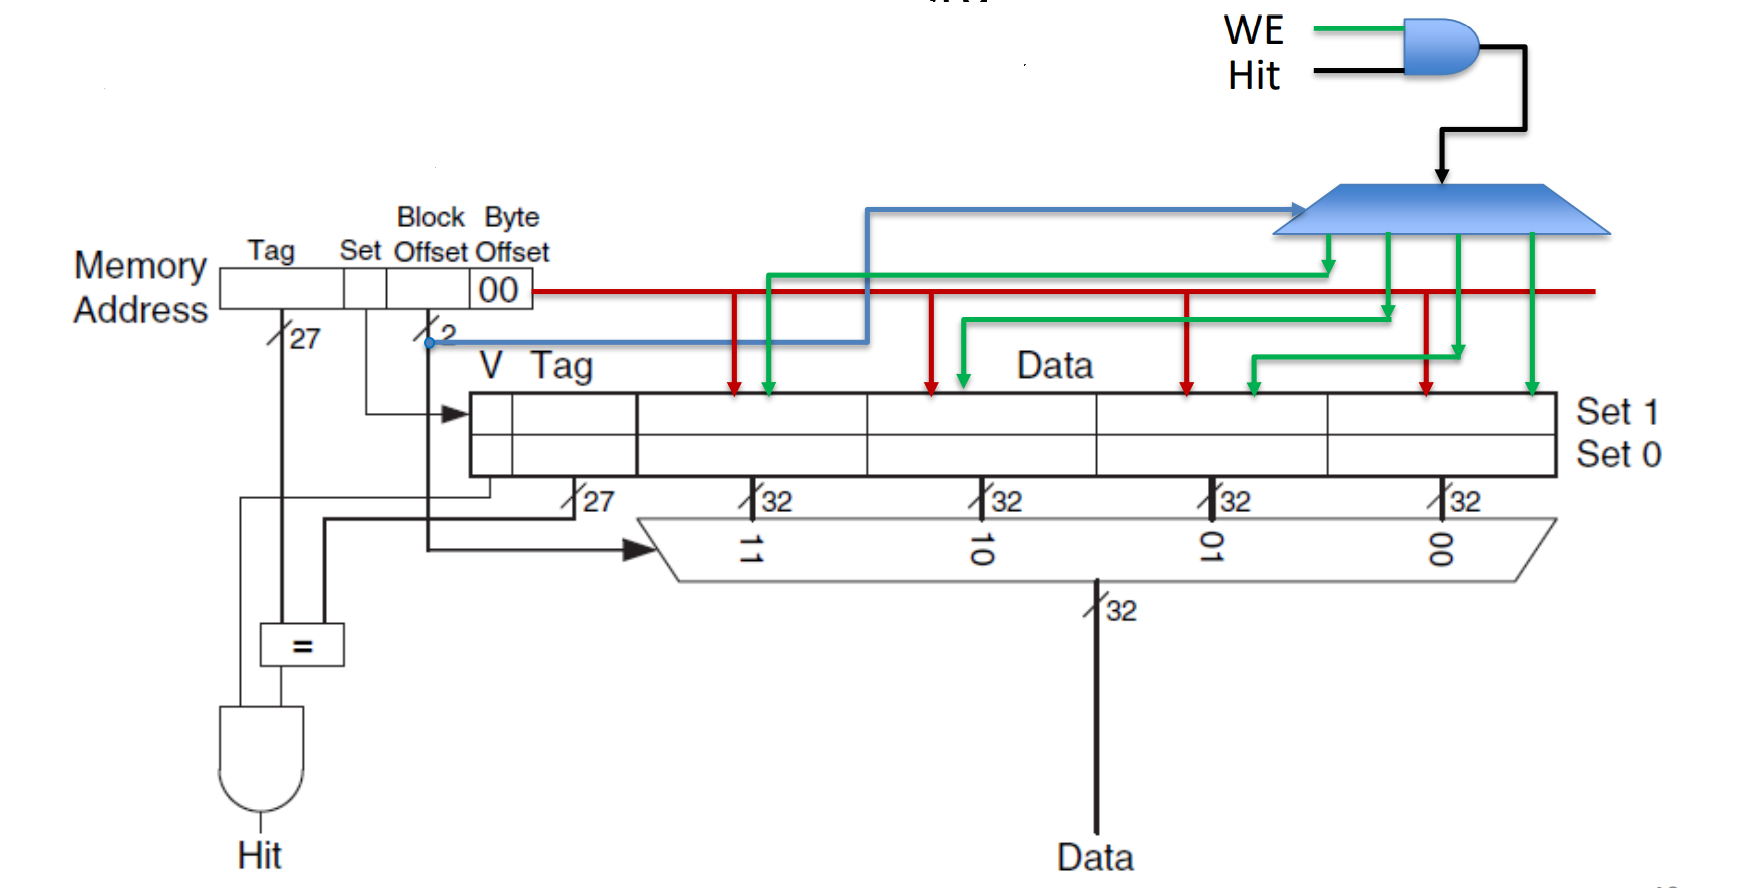
\includegraphics[scale=0.15]{images/direct_mapped_3.png}
\end{center}

\begin{example}
	\label{example:direct_access_1}
	Supponiamo di avere indirizzi a $32$bit, una cache ad accesso diretto con $S = B = 128$ ed ognuna contiene $b = 8$. Dobbiamo trovare la struttura con cui organizzare gli indirizzi.\\
	Ci servono $2$bit per l'offset del dato, $log_2 8=3$bit per l'offset delle parole nel blocco, \(\log_2 129 = 7\)bit per identificare il \emph{set} e 20bit per il tag del dato.
	\begin{center}
		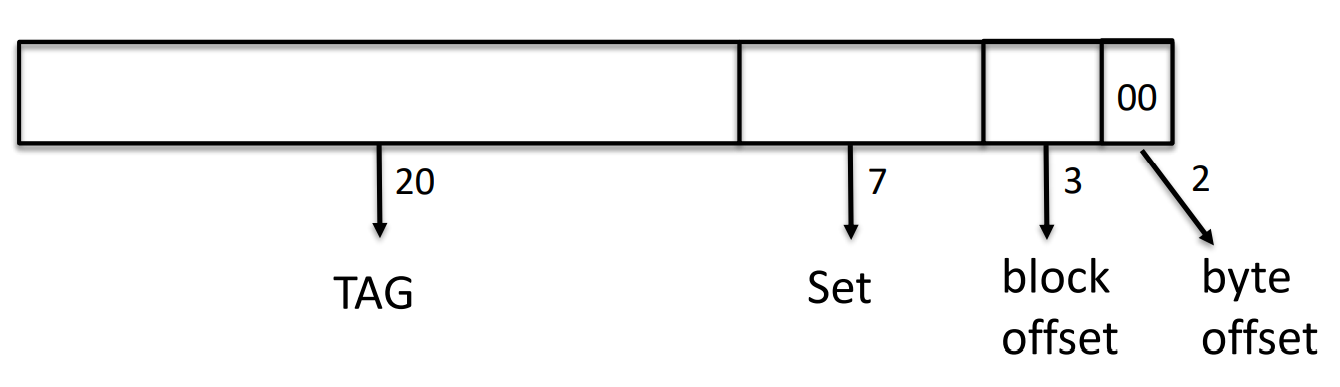
\includegraphics[scale=0.1]{images/direct_mapped_example_1.png}
	\end{center}
\end{example}

\begin{example}
	Consideriamo la stessa struttura dell'esempio \ref{example:direct_access_1}. Dobbiamo calcolare la linea di cache e l'offset all'interno della linea
	di cache che conterrà l'indirizzo 0xFFAC.\\
	\begin{equation*}
		\text{0xFFAC} = 0\ldots01111 \color{red}1110 101\color{green}0 11\color{blue}00\color{black} 
	\end{equation*}
	L'indirizzo si dividerà quindi in:
	\begin{itemize}
		\item Tag
		\item \color{red}Set\color{black}
		\item \color{green}Block offset\color{black}
		\item \color{blue}Byte offset \color{black}
	\end{itemize}
	Quindi la linea di cache ha indice 117, ovvero 118esima. L'offset nel blocco è 3 quindi la quarta parola di memoria.
\end{example}

\begin{example}
	Consideriamo il seguente codice in C:
	\begin{lstlisting}[language=C]
		for(i=0; i<16, i++)
		C[i] = A[i] + B[i];
	\end{lstlisting}
	eseguito in un processore a 2Ghz con un mapping diretto L1 ai dati dalla cache con $C = 128$, $b=8$, \(t_M = 100\) cicli e \(t_{L1} = 4\) cicli.\\
	'A' inizia all'indirizzo 0x00000000, 'B' inizia all'indirizzo 0x00000040 e 'C' inizia all'indirizzo 0x00000080. Calcolare il numero di cache misses e l'AMAT considerando solo le \emph{ldr}.\\\\
	Il primo passo è verificare se A e B finiscono nello stesso set: A verrà caricato nel set 0 e nel set 1 mentre B nel set 2 e nel set 3, quindi non vanno in conflitto.
	Se supponiamo la cache sia vuota: avremo 4 cache misses, due per ogni word di A e B, e 32 cache hits (12 per A e 12 per B).\\
	Il calcolo dell'AMAT sarà
	\begin{equation*}
		\begin{split}
			&MissRate = \frac{4}{32}\\
			&CloclCycleTime=\frac{1}{2GHz}=0.5ns\\
			&AMAT=\bigg(4+\frac{4}{32} \cdot 100\bigg) \cdot ClockCycleTime = 8.25ns
		\end{split}
	\end{equation*}
	In generale, se non c'è \textbf{località temporale}, il numero di cache misses è $\frac{N}{b}$, dove $N$ è il numero di istruzioni (in questo caso $N=2\cdot16$).
\end{example}

\noindent Per riassumere possiamo dire che i pro sono:
\begin{itemize}
	\item La realizzazione è semplice
	\item E' molto veloce in caso di hits
\end{itemize}
mentre i contro:
\begin{itemize}
	\item La funzione di mapping a posizione fisse può generare potenzialmente molti conflitti.
	\item La troppa rigidità potrebbe avere un grosso impatto sul numero dei conflitti nella cache (\textbf{trashing}) in quanto essi dipendono dal posizionamento della memoria e dall'utilizzo delle strutture dati.
\end{itemize}

\begin{definition}[Working set]
	Data una gerarchia di memoria M1-M2, il working set di un programma è l'insieme dei dati che, se simultaneamente presenti in M1, massimizza la probabilità di hits in M1.
\end{definition}

\begin{example}[Working set]
	Prendiamo per esempio il seguente codice:
	\begin{lstlisting}[language=C]
		// A and B are two arrays of size N
		// (the cache block b << N)
		for(i=0; i<N; ++i)
		for(j=0; j<N; ++j)
		A[i] = F(A[i], B[j])
	\end{lstlisting}
	in cui l'array A ha località spaziale e temporale e B quella spaziale (sul lungo termine anche temporale).\\
	Il nostro WS sarà l'elemento corrente di A e l'intero array B. Quindi, se la cache contenesse il WS avremmo solamente $O(\frac{N}{b})$ fallimenti.
\end{example}

\subsubsection{Associative}
Esistono due tipi di cache associative:
\begin{itemize}
	\item \textbf{Fully associative}: i blocchi possono essere posizionati in qualunque \emph{cache line}. Per trovarlo bisogna scansionare tutte le linee; questo implica un comparatore per ogni linea (più costoso).
	\item \textbf{Set associative}: i blocchi possono essere posizionati in un certo numero di set, dove ogni set contiene un certo numero di linee che possono essere utilizzate indiscriminatamente (purché del set giusto).
\end{itemize}

\begin{figure}[h!]
	\centering
	\begin{subfigure}{.45\textwidth}
		\centering
		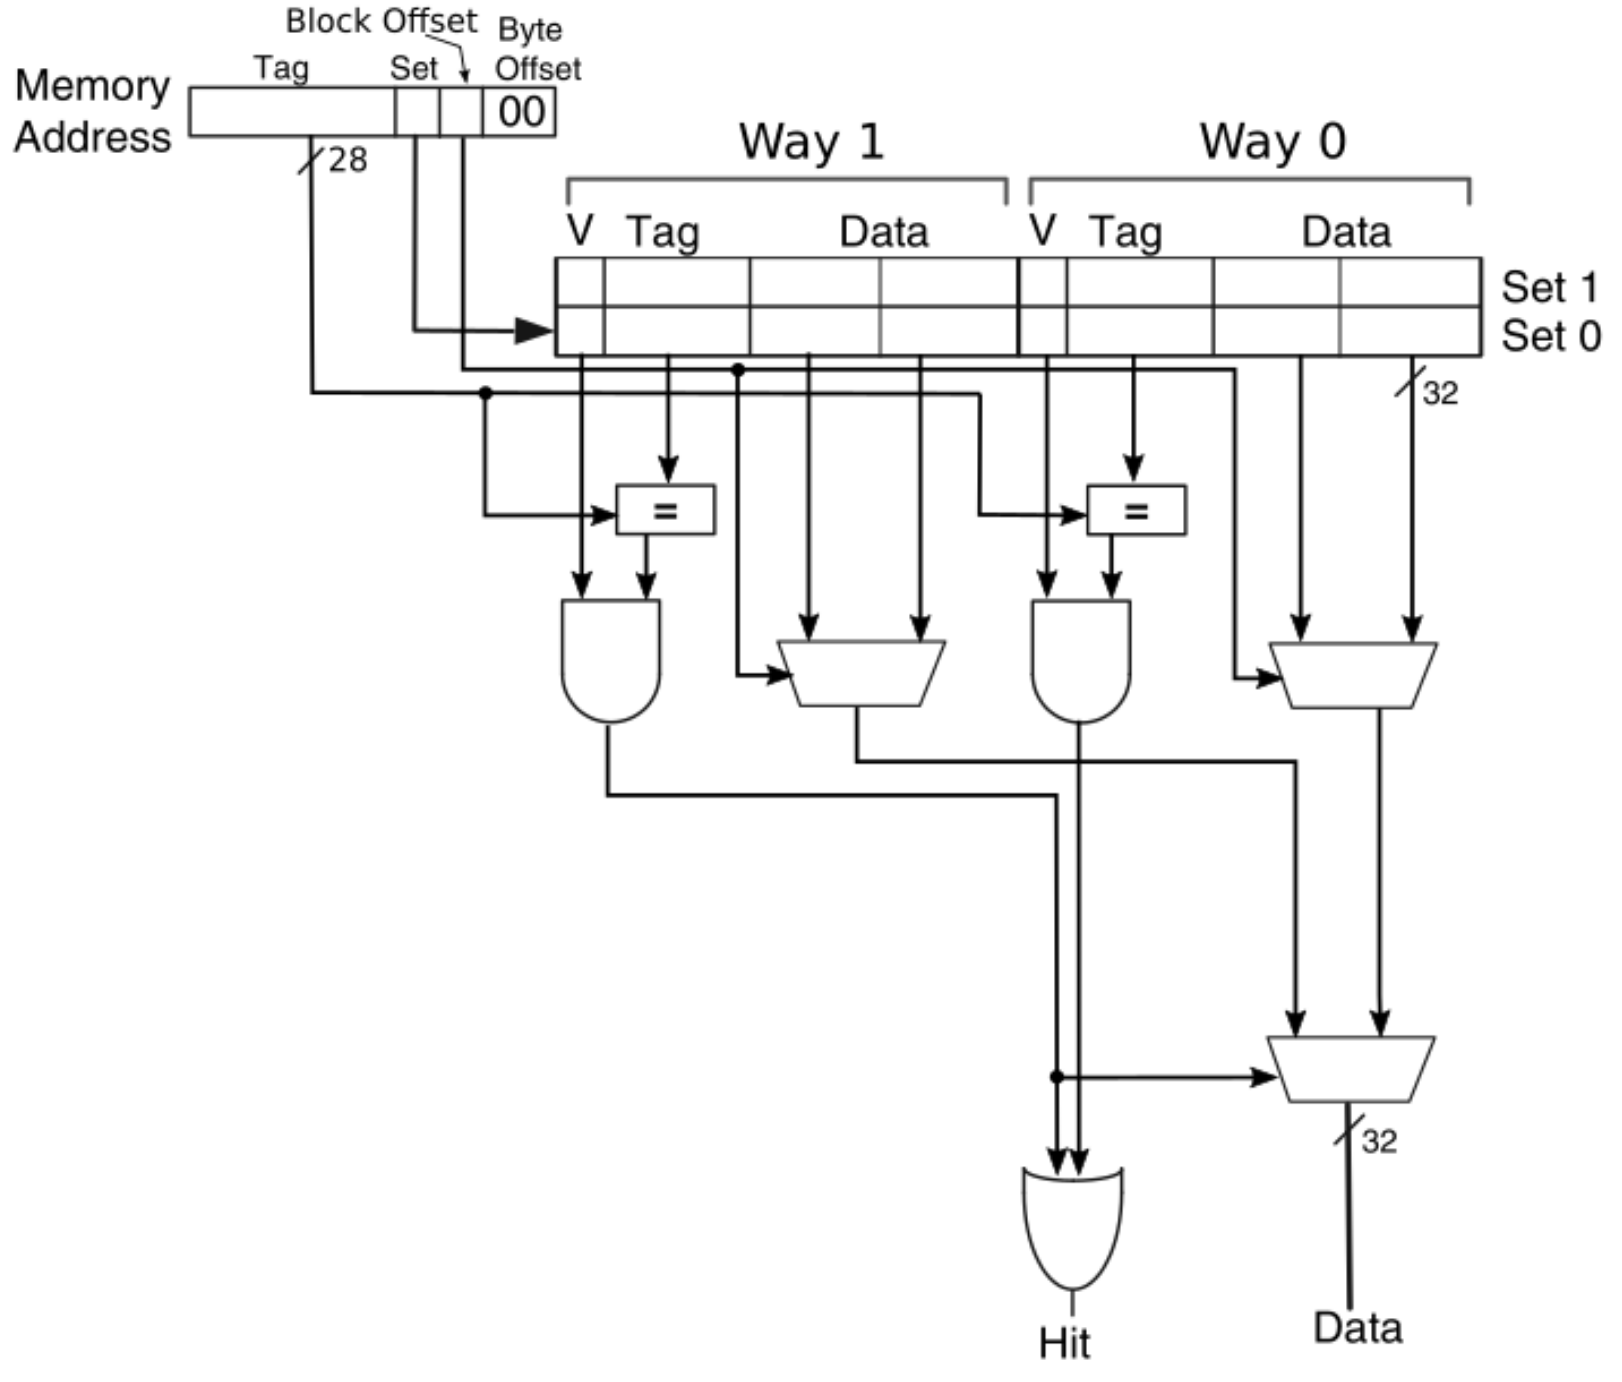
\includegraphics[width=4.7cm]{images/fully-associative.png}
		\caption{Fully associative}
	\end{subfigure}
	\begin{subfigure}{.45\textwidth}
		\centering
		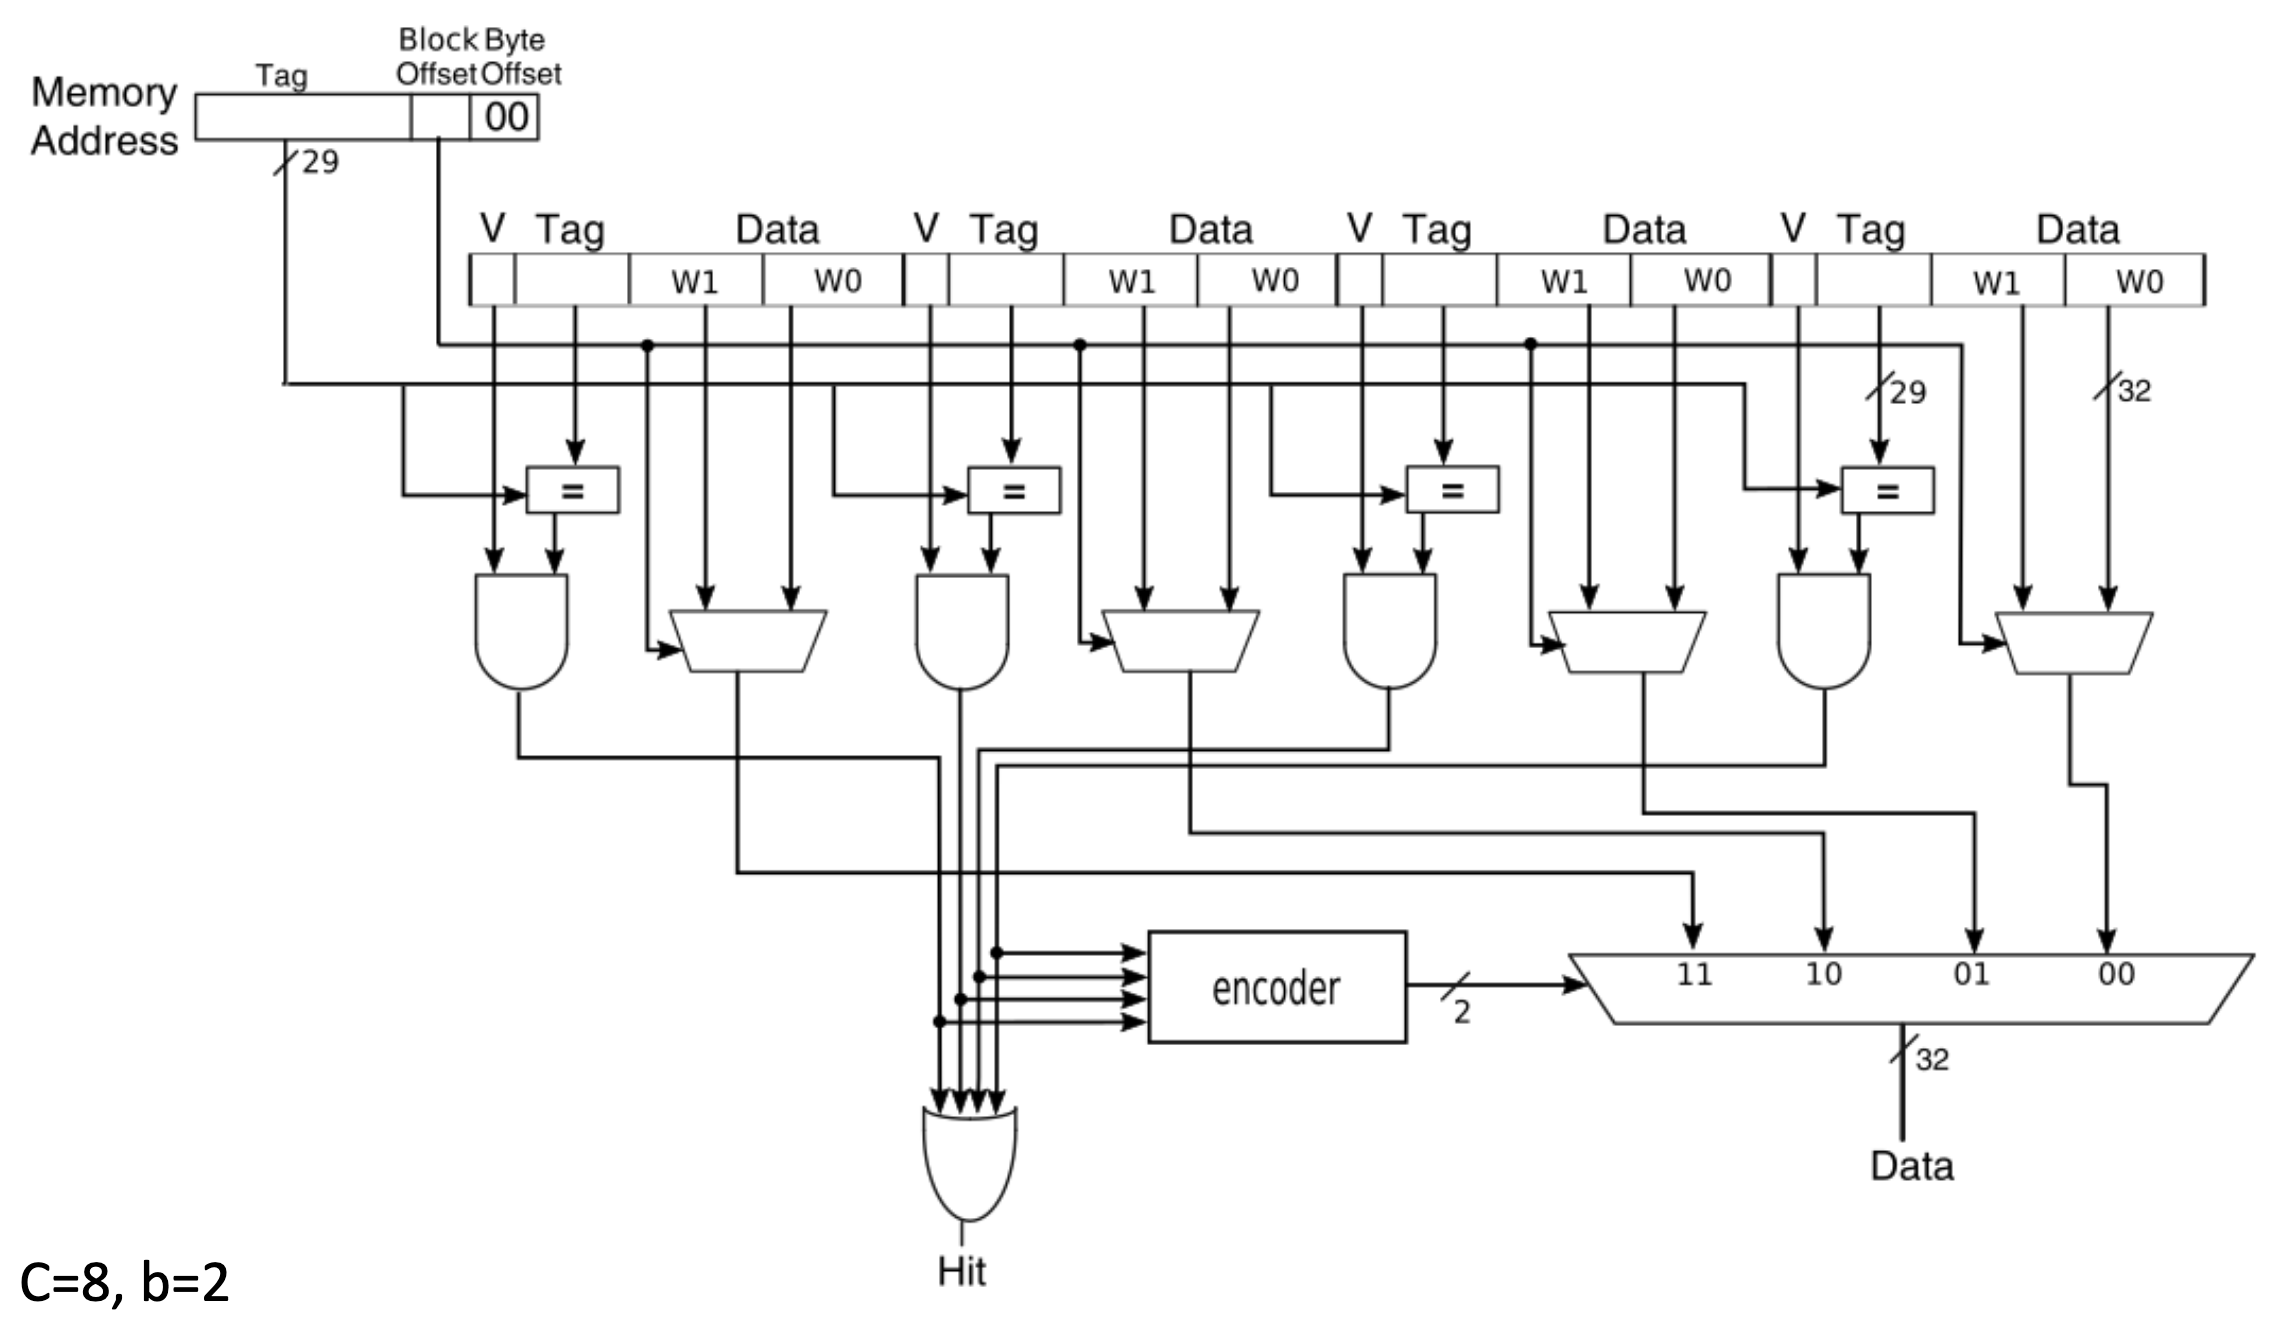
\includegraphics[width=4.7cm]{images/n-way-associative.png}
		\caption{N-way associative}
	\end{subfigure}
\end{figure}

\subsubsection{Comparazione}
Data una capacità $C$, dobbiamo decidere la dimensione del blocco $b$, il numero di blocchi $B$ (cache lines, $\frac{C}{b}$) e il numero di vie (numero di blocchi in un Set).
\begin{table}[h]
	\centering
	\begin{tabular}{|c|c|c|}
		\hline
		Organizzazione & Numero di vie $N$ & Numero di Set $S$ \\
		\hline
		Direct mapped & 1 & $B$ \\
		Set associative & $1<N<B$ & $\frac{B}{N}$ \\
		Fully associative & $B$ & 1\\
		\hline
	\end{tabular}
\end{table}

\subsection{Cache miss}
Le tipologie di cache miss sono le seguenti:
\begin{itemize}
	\item \textbf{Compulsory miss}: causato dal primo acceso al blocco che non è mai stato in cache.
	\item \textbf{Capacity miss}: causato dalla cache che non contiene tutti i blocchi necessari.
	\item \textbf{Conflict miss} solo per la mappatura diretta e per i set associativi
\end{itemize}
A questo punto, visti i vari strumenti della cache e le tipologie di miss possiamo vedere come ridurre i cache miss tramite l'utilizzo di alcune tecniche:
\begin{itemize}
	\item \textbf{Aumentare la dimensione dei blocchi}. Andando così ad aumentare la località spaziale ma aumentando anche la \textbf{miss penalty}.
	\item \textbf{Aumentare l'associatività}. Meno conflitti ma un maggiore tempo di hit.
	\item \textbf{Aumentare dim. dei case}. Porta a meno capacity miss e conflitti ma aumenta l'hit time.
	\item Usare algoritmi \textbf{cache-oblivious} per sfruttare al massimo la località.
\end{itemize}
\begin{figure}[h]
	\centering
	\begin{subfigure}{.45\textwidth}
		\centering
		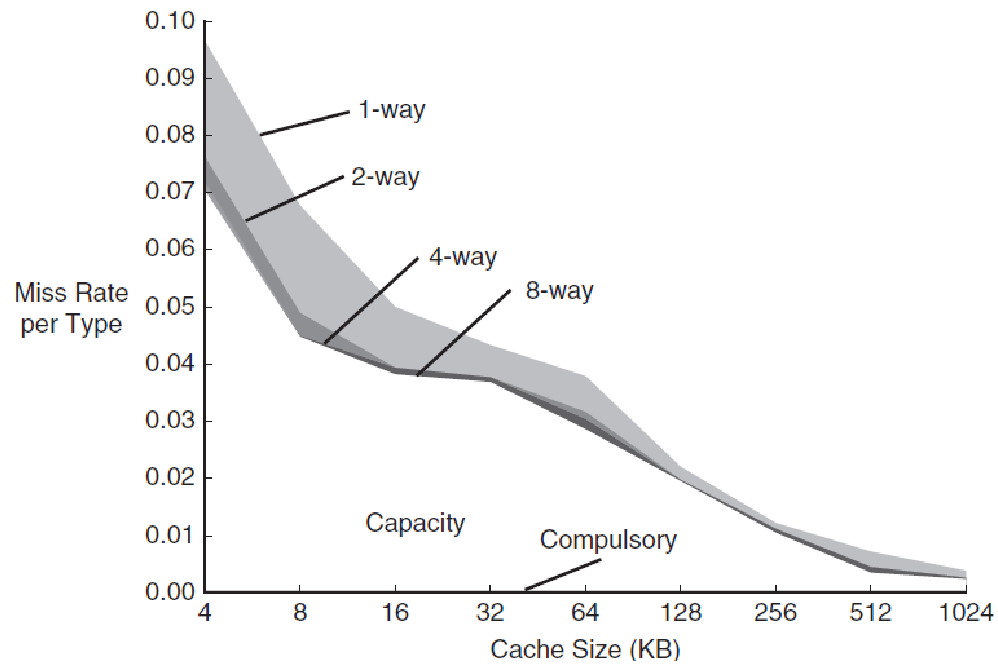
\includegraphics[width=4.7cm]{images/miss_rate_cache_size.png}
		\caption{Aumentare dimensione cache e associatività}
	\end{subfigure}
	\begin{subfigure}{.45\textwidth}
		\centering
		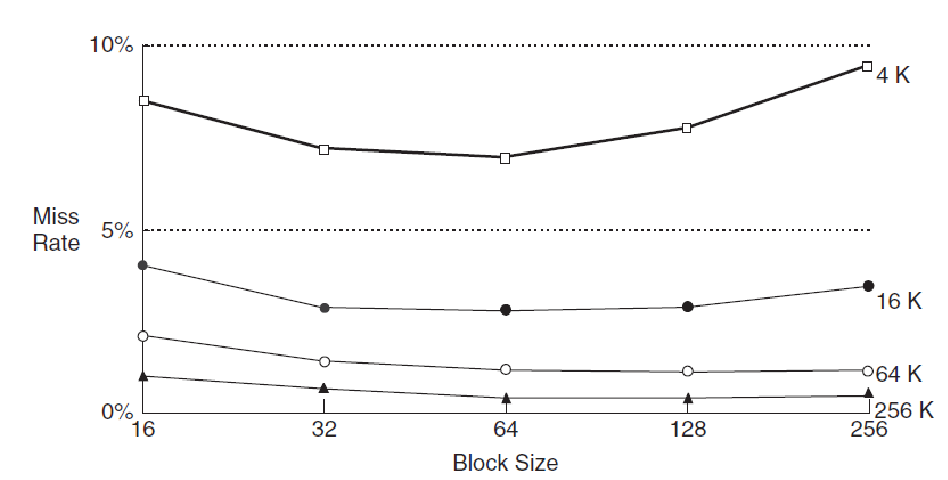
\includegraphics[width=4.7cm]{images/miss_rate_block_size.png}
		\caption{Aumentare la dimensione dei blocchi}
	\end{subfigure}
\end{figure}

In caso comunque avvengano dobbiamo andarli a gestire. Un errore nella cache blocca l'intero processore, congelando il contenuto di tutti i registri durante l'attesa della memoria: in effetti, un processore più avanzato consente l'esecuzione fuori ordine di altre istruzioni durante l'attesa della memoria.
Gli steps che vengono eseguiti per la gestione di un cache miss (\textbf{fault management}):
\begin{enumerate}
	\item Indica al livello di memoria successivo nella gerarchia di leggere il valore mancante.
	\item Attende che la memoria risponda (questo può richiedere più cicli).
	\item Aggiorna la riga della cache corrispondente con i dati ricevuti.
	\item Riavvia l'esecuzione dell'istruzione (ora è un hit della cache).
\end{enumerate}

\begin{example}[Migliorare performance della CPU]
	Partiamo dal caso dell'esempio \ref{example:cache_performance} e supponiamo di raddoppiare la velocità di clock:
	\[CPI_{Stall-Instr} = 1 \cdot 0.02 \cdot 200 = 4 cycles\]
	\[CPI_{Stall-Data} = 0.36 \cdot 0.4 \cdot 200 = 2.88 cycles\]
	\[CPi_{stall} = 4 + 2.88 = 6.88\]
	\[CPI = 2+6.88 = 8.88\]
	Il tempo che stiamo fermi in attesa della memoria cresce al $77\%$:
	\begin{equation*}
		\frac{6.88}{8.88}=0.77
	\end{equation*}
	e abbiamo quindi un miglioramento totale di un fattore di solo:
	\begin{equation*}
		\frac{CPU_{time1}}{CPU_{time2}} = \frac{(CPI_Perf + CPI_{Stall1}) \cdot ClockCycleTime}{(CPI_Perf + CPI_{Stall2}) \cdot \frac{ClockCycleTime}{2}} = \frac{5.44}{\frac{8.88}{2}} = 1.23
	\end{equation*}
\end{example}
Come si vede da questo esempio, migliorare la velocità del processore o la sua architettura non migliora in maniera efficiente il tempo impiegato nell'attesa della memoria, che per l'esempio è relativamente di
\begin{equation*}
	\epsilon = \frac{1.23}{2}=61\%
\end{equation*}
\subsubsection{Multi-level cache}
Per ovviare a questo problema vengono utilizzate cache su più livelli, dove quelle dei livelli inferiori vengono interrogate in caso di cache miss ed evitano quindi un accesso alla memoria principale (che si rende necessario solo se non si trova il dato neanche sull'ultimo livello).
\begin{example}[Multi-level cache]
	%TODO Da aggiungere
\end{example}

\begin{example}
	Considera una piccola cache con $4$ blocchi, $b=1$. Trova il numero di miss per una cache direct-ampped per la seguente sequenza ordinata di indirizzi di blocco: 0, 8, 0, 6, 8.
	\begin{table}[h]
		\centering
		\begin{tabular}{|c|c|}
			\hline
			Block address & Cache block \\
			\hline
			0 & $0 \% 4=0$ \\
			6 & $6\% 4 = 2$\\
			8 & $8\%4=0$\\
			\hline
		\end{tabular}
	\end{table}
	\begin{table}[h]
		\centering
		\begin{tabular}{|c|c|c|c|c|c|}
			\hline
			\multirowcell{2}{Address} & \multirowcell{2}{Hit or miss} & \multicolumn{4}{c}{Contents after reference} \\
			\hline
			%TODO Sistema e aggiungi gli altri esempi
			\hline
		\end{tabular}
	\end{table}
\end{example}

\subsection{Gestione delle scritture}
Distinguiamo le scritture in due casi:
\begin{itemize}
	\item \textbf{Write hits} quando c'è lo stesso TAG: se il dato viene scritto solo nella cache, allora la memoria e la cache sono inconsistenti
	\item \textbf{Write miss} quando abbiamo tag diversi
\end{itemize}

\subsubsection{Write-Through}
Questa tecnica prevede che gli hit di scrittura aggiornino sempre sia la cache che il successivo livello di memoria.
\begin{itemize}
	\item \textbf{Pro}: soluzione \textbf{semplice}, facile da implementare. I dati sono sempre coerenti tra i due livelli di memoria.
	\item \textbf{Contro}: la \textbf{velocità} di scrittura dipende dalla velocità di scrittura del livello di memoria inferiore. Maggiore \textbf{traffico di memoria}, per ogni singola scrittura potrebbero esserci più scritture in ogni livello di memoria.
\end{itemize}

\subsubsection{Write-Back}
Gli hit di scrittura aggiornano solo la cache, quindi il blocco modificato viene scritto nel livello di memoria inferiore quando viene sostituito. 
\begin{itemize}
	\item \textbf{Pro}: la \textbf{velocità} delle scritture è quella della cache: minore traffico di memoria rispetto a Write-Through, le successive scritture sullo stesso blocco di cache non producono traffico con il livello di memoria inferiore più costoso.
	\item \textbf{Contro}: 
	Abbiamo bisogno di tenere traccia dei blocchi modificati (bit sporchi). Più \textbf{complesso} da implementare rispetto al Write-Through. La sostituzione della riga della cache è più costosa.
\end{itemize}

\begin{example}
	Supponiamo che una cache abbia un blocco di 4 parole. Quanti accessi alla memoria principale sono necessari in base alle due politiche di accesso per il seguente codice?
	\begin{lstlisting}[language={[x86masm]Assembler}]
		MOV R5, #0
		STR R1, [R5]
		STR R2, [R5, #12]
		STR R3, [R5, #8]
		STR R4, [R5, #4]
	\end{lstlisting}
	Tutte e 4 le istruzioni scrivono sullo stesso blocco di cache. Con la tecnica \textbf{write-through}, ogni istruzione scrive nella memoria principale e richiede quindi 4 scritture. Con la tecnica write-back serve solamente un accesso alla memoria principale per pulire il blocco.
\end{example}

Il \textbf{write-back} può migliorare le prestazioni specialmente quando la CPU genera istruzioni di memorizzazione più velocemente di quanto la memoria principale può gestire, tuttavia, il costo delle scritture nella cache è maggiore se si verifica un errore di scrittura, dobbiamo prima riscrivere il blocco in memoria (se il dirty bit è 1). 
Ciò richiede almeno due cicli anche per un hit di scrittura: un ciclo per verificare un hit seguito da un ciclo per eseguire effettivamente la scrittura. In alternativa, possiamo usare un buffer di scrittura per trattenere temporaneamente i dati da scrivere mentre il blocco della cache è controllato per un colpo. 
Il processore esegue la ricerca nella cache e inserisce i dati nel buffer di scrittura durante il normale ciclo di accesso alla cache. Supponendo un riscontro nella cache, i nuovi dati vengono scritti dal buffer di scrittura nella cache al successivo ciclo di accesso alla cache inutilizzato (pipelining degli accessi).

\subsubsection{Ottimizzare le scritture}
Poiché la scrittura nella memoria off-chip è costosa, gli archivi di memoria sono bufferizzati, un \textbf{buffer di scrittura} viene utilizzato per conservare i dati in attesa di essere scritti nella memoria.
L'esecuzione continua immediatamente dopo la scrittura dei dati nella cache e nel buffer di scrittura, i salvataggi nella nella memoria principale vengono eseguiti in parallelo con il calcolo della CPU. 
La CPU va in stallo solo se il buffer di scrittura è pieno, quindi la larghezza di banda richiesta dalla memoria principale è un fattore critico, in particolare per il modello di cache Writhe-Through.

\subsection{Cache replacement}
In una direct mapped cache, il blocco richiesto può andare esattamente in una posizione, quindi non abbiamo scelta: 
se il blocco da sostituire è stato modificato e la politica di scrittura è Write-Back, dobbiamo aggiornare la memoria di livello inferiore. 
Con la cache associativa, possiamo scegliere dove posizionare il blocco richiesto: 
\begin{itemize}
	\item \textbf{Fully associative} cache, tutti i blocchi sono candidati per la sostituzione.
	\item \textbf{N-way set-associative} cache, dobbiamo scegliere tra gli Nblocchi nel set selezionato.
\end{itemize}

%TODO Ti sei perso

\subsubsection{Cache replacement policy}
Per decidere quali blocchi rimpiazzare dobbiamo distinguere per i tipi di cache:
\begin{itemize}
	\item \textbf{Direct mapped}: se il blocco da rimpiazzare è stato modificato e usiamo una policy di \textbf{write-back} dobbiamo aggiornare la memoria di livello più basso
	\item \textbf{Associative cache}:
	\begin{itemize}
		\item  \emph{Fully associative}: tutti i blocchi sono candidati per essere sostituiti
		\item \emph{N-way set-associative}: dobbiamo scegliere tra gli $N$ blocchi nel set selezionato
	\end{itemize}
\end{itemize}
Lo schema più utilizzato è \textbf{Least Recent Used (LRU)}. Sfrutta la località temporale: il blocco sostituito è quello che è rimasto inutilizzato per il tempo più lungo. 
Per una cache set-associativa a 2 vie, può essere implementato con 1 bit (usare bit --U), per un 4 vie è ancora fattibile con 2 bit, per più di 4 vie diventa abbastanza complicato (pseudo-LRU).
Per le cache altamente associative, una politica \textbf{Random} offre all'incirca le stesse prestazioni di LRU.

\subsection{Designing the Memory System}
La miss penalty può essere ridotta aumentando la larghezza di banda del bus tra DRAM e cache. Ci sono tre possibili organizzazioni:
\begin{itemize}
	\item \textbf{Semplice}: una parola alla volta viene letta dalla memoria.
	\item \textbf{Ampia memoria}: N parole alla volta vengono lette dalla memoria.
	\item \textbf{Interleaved}: K banchi di memoria indipendenti in grado di servire K richieste contemporaneamente.
\end{itemize}
Consideriamo il tempo di trasferimento del blocco della cache per l'organizzazione della memoria Simple contro quella Interleaved.\\
Il caso \textbf{semplice} è il seguente:
\begin{center}
	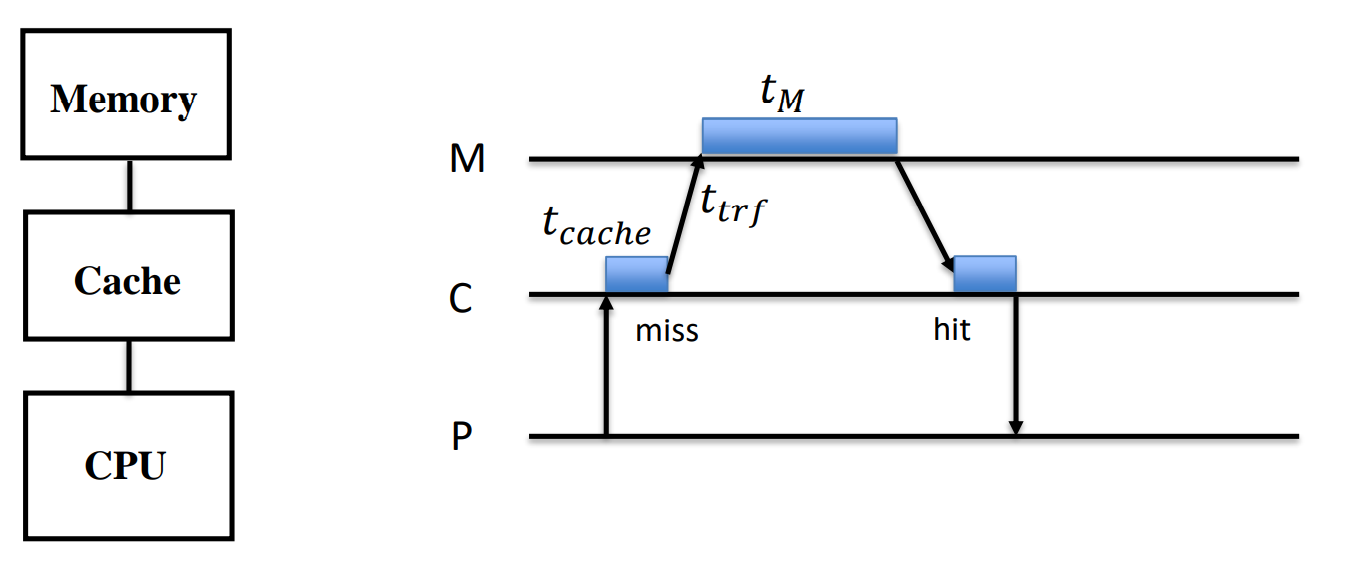
\includegraphics[scale=0.2]{cache_block_transfer.png}
\end{center}
Sapendo che il memory time e il cache time sono rispettivamente $t_M$ e $t_{cache}$, la larghezza di banda della memoria sarà $B_M = \frac{1}{t_M}$ e $b=1$. Il memory access time è
\begin{equation*}
	t_a=2 \cdot t_{trf} + 2 \cdot t_{cache} + t_M
\end{equation*}
Se la cache line contiene più di un blocco, il suo costo di trasferimento in caso di cache miss sarà
\begin{equation*}
	t_{miss}=2 \cdot t_{trf} + 2 \cdot t_{cache} + b \cdot t_M \approx b \cdot t_M
\end{equation*}

\begin{example}
	Se consideriamo $b=8$, $t_M =80$, $t_{cache}=1$ e $t_{trf}=6$ cicli di clock, allora il costo del cache miss sarà molto alto, circa $>650$ cicli di clock.
\end{example}
Invece per quanto riguarda il caso \textbf{interleaved}:
\begin{center}
	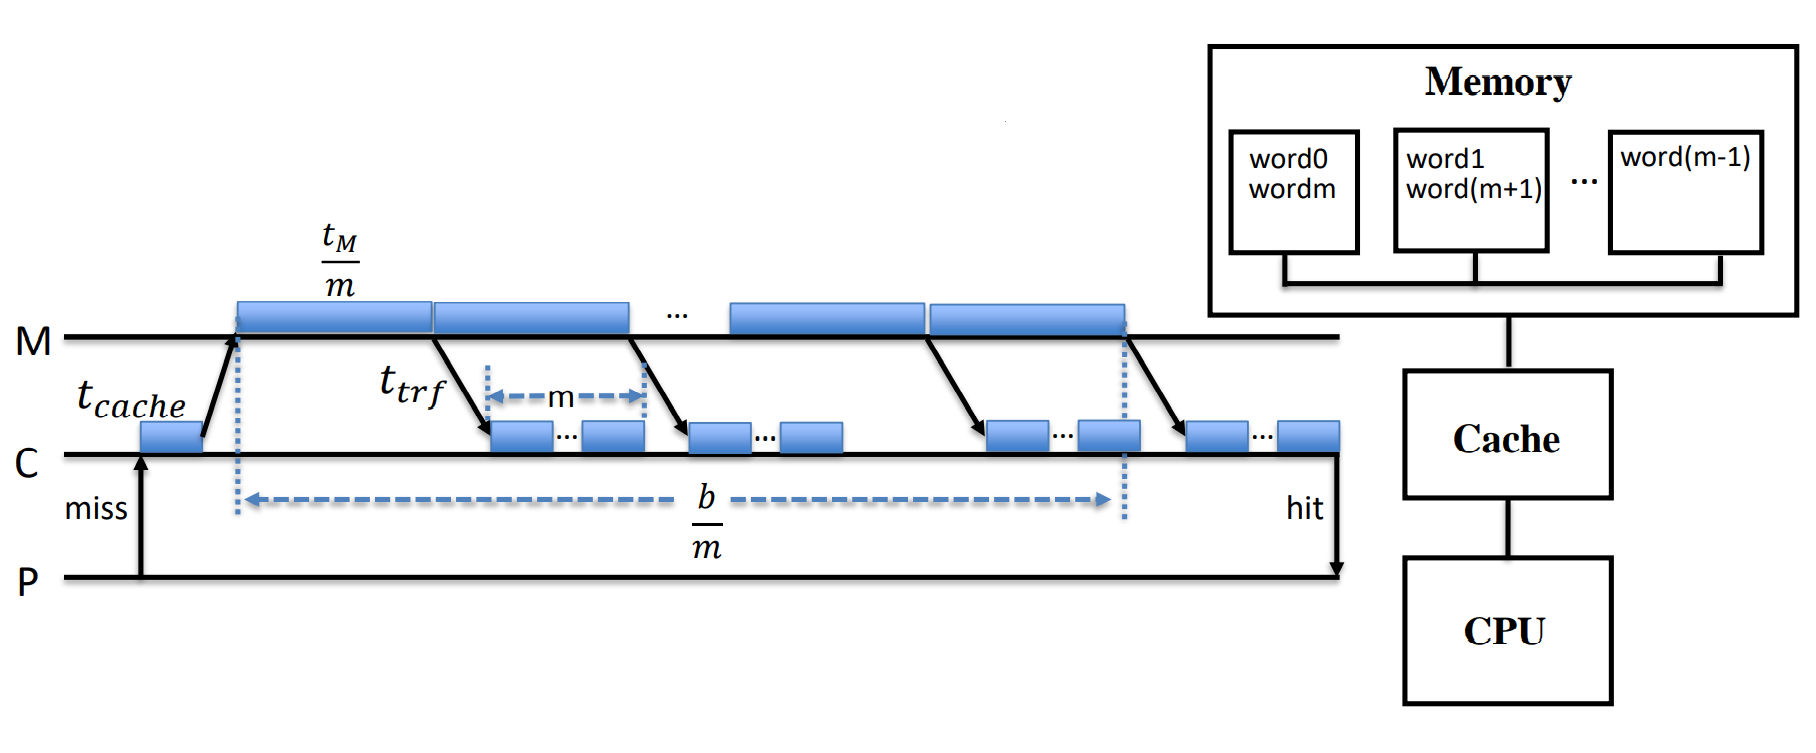
\includegraphics[scale=0.2]{cache_block_transfer_interleaved.png}
\end{center}
aumentiamo la larghezza di banda di un fattore del numero di moduli $m$
\begin{equation*}
	B_M = \frac{m}{t_M}
\end{equation*}
avendo quindi un costo di
\begin{equation*}
	t_{miss}=2 \cdot t_{trf} + (\sim 1 + 1) \cdot t_{cache} + \frac{b}{m} \cdot t_M \cdot t_M
\end{equation*}
che, se poniamo $b=m$, diventa $t_{miss} \approx t_M$.

\subsection{Problemi cache}
La memorizzazione nella cache è essenziale per ridurre il collo di bottiglia di von Neuman e ottenere prestazioni ragionevoli sui sistemi moderni. Tuttavia, la memorizzazione nella cache introduce alcuni problemi nei sistemi multiprocessore/multicore.\\ 
Problema di \textbf{coerenza} della cache e \textbf{falsa condivisione} (due variabili non correlate sono collocate nello stesso blocco della cache e accesso in modalità lettura/scrittura da thread diversi).

\subsubsection{Problemi di corerenza}
Supponiamo un'architettura SMP (Symmetric Multiprocessors), ovvero con caching di dati privati e condivisi. I dati core privati vengono memorizzati nella cache in L1, riducendo così l'AMAT e le comunicazioni di memoria off-chip. 
Quando i dati condivisi vengono memorizzati nella cache, i valori condivisi possono essere replicati in più core cache private, riducendo anche la contesa di memoria. Cosa succede se i dati condivisi vengono scritti? \\
Viene introdotto un nuovo livello dell'architettura che forza a mantenere la consistenza dei dati per linee diverse di cache. Uno dei protocolli più semplici è il \textbf{write invalidate}, che consiste nell'invalidare tutte le altre linee di cache non aggiornate tramite un bus di tipo \emph{snoopy}. Esistono anche protocolli di aggiornamento ma sono più complicati.